%\input{chap1/introduction.tex}

\setcounter{chapter}{0}

\chapter{Introduction}\label{cha:introduction}

In this chapter, we introduce the context of our research, which falls in the area of agent communication within Multi-Agent Systems (MASs). More precisely, it is concerned with modeling and verifying social commitments --as a means of communication among agents-- in the presence of probabilistic behavior. We also identify the motivations, problem statement, and research questions that we address in this thesis. Then, we list our objectives and discuss our methodology. Finally, we conclude this chapter by providing the thesis outline.


\section{Context of Research} \label{sec:context-chap1}

\subsection{Multi-Agent Systems (MASs)}
Nowadays, the use of distributed environments to solve complex
real world problems using entities called agents is on rise
\cite{Biswas08,Park2005}. Agents are active, social, and adaptable computer systems situated in some dynamic environment and capable of autonomous actions \cite{Wooldridge2009}. %to achieve their objectives \cite{Wooldridge2009}. %To attain their objectives, agents need abilities to cooperate, coordinate, and negotiate.
Ideally, an agent has to be \cite{Wooldridge1995}:

\begin{itemize}
\item Reactive: able to respond to changes in its environment.
\item Pro-active: capable to behave with respect to its goals (goal-directed behavior).
\item Social: able to interact and communicate with others.
\item Autonomous: able to operate without direct intervention of others.
\end{itemize}

In addition to being autonomous, agents are possibly heterogeneous; that is, agents may be independently designed by different programmers and hence it is difficult to make assumptions about their present or future behavior.
A multi-agent system (MAS) consists of a set of these autonomous
entities, which interact with each other and their
surrounding environment to achieve their (joint) objectives
\cite{Wooldridge2009}. In an open system, autonomous agents can freely enter and exit different interactions at any time \cite{Fornara2004a}. In principle, open MASs provide no guarantees about the behavior of their agents. This means that when agents are working together, such as carrying out a business protocol, an agent's misbehavior may potentially create an
exception for another agent and obstruct its proper working.
However, one can look at multi-agent systems from different
perspectives. From the computing perspective, a MAS is a
computational paradigm and an advance in computer science. From
the software engineering perspective, multi-agent technology is a
new software engineering paradigm providing new abstractions for
different phases of software development process. MASs approaches
can be seen as very efficient and modular ways of modeling and
implementing systems as they are capable of designing and
programming autonomous agents with different abilities, behaviors,
and intentions. From the artificial intelligence perspective, MASs
provide better understanding and modeling of social intelligence
and emergent behaviors.



\subsection{Agent Communication Languages (ACLs)}
Communication is a fundamental aspect for autonomous agents in MASs to coordinate with one another to solve complex problems that are difficult for an individual agent to tackle. Therefore, communication among agents is a key element to build effective MASs. In many realistic settings, agents need to interact to realize their goals. The type of interaction among the agents varies according to the goals of these interacting parties and the context of the transactions they are performing. An agent may cooperate with other agents to perform a certain task, compete with others to achieve a shared goal, or do a combination of both in order to perform individual or group tasks.

The importance of defining a standard framework for agent communication has been widely recognized. However, there have been many attempts in the literature to agree on standards for agent communication. Semantics of ACLs are defined either internally (privately) in terms of agents' beliefs and goals, or externally (publicly) in terms of agents' social commitments.
%Communication between agents are %governed by means of protocols. Roughly speaking, a protocol %determines which messages can be exchanged and in which order.
Approaches defined using the former type of semantics are called mental
approaches because they focus on the minds of interacting agents, while those defined using the latter one are called social approaches because they consider the social context of the interacting parties. In contrast to mental approaches such as those that are built using FIPA-ACL\footnote{See FIPA-ACL (Foundation for Intelligent Physical Agents - Agent Communication Language) specifications (1997,1999,2001,2002), http://www.fipa.org/repository/aclspecs.php3} and KQML (Knowledge Query and Manipulation Language) \cite{Finin1994}, social commitments proved to be a powerful representation for agent interactions \cite{Bentahar2010,Mallya2007,Yolum2004}. They provide a social semantics that abstracts away from the agents internal states and offers social and observable meaning to the messages being exchanged among agents. In the context of this thesis, we focus on the kind of communication in which the semantics of messages is defined publicly, i.e., in terms of social commitments.



\section{Motivations} \label{sec:Motivations-chap1}
Our review of the social commitments literature has revealed a gap in handling probabilistic social commitments in MASs. We have noticed that though social commitments have been the subject of a vast research activity for more than a decade, current proposals to represent and verify social commitments, for instance \cite{Bentahar2012,Bentahar2009,Bentahar2004,Colombetti2000,Colombetti2004,El-Menshawy2010,El-Menshawy2013a,Singh2000,Verdicchio2003}, assume typical settings in which agents behave in an ideal manner, and consequently commitments among interacting agents are treated under the assumption of certainty. However, in the formulation of agent-based systems, the role of uncertainty is crucial for an efficient and coherent resolution of complex problems. Simply put, agents in MASs overcome complex problems thanks to their individual capabilities to be autonomous and to adapt their behavior with the changing of the environment in which they live and
interact. Practically speaking, agents cannot always observe all the changes in the environment, but instead each agent can only have a partial view of other agents' behavior \cite{Gammie2004}. Indeed, the presence of imperfect information about the environment leads autonomous agents to make estimations about the observable world as part of their autonomous decision making processes \cite{Walley1996}. This means that agents inevitably meet uncertainty during their work, or in many cases, for the high complexity of the problem, the information they handle is (or needs to be) approximate.


This unpredictable behavior of MASs raises different important questions. The interesting issue that we are mainly focusing on is how social commitments can be tackled in such systems. In reality, due to agents' autonomy, a request to create a social commitment is not always followed by the creation of that commitment. The same principle applies to fulfilling an established commitment. That is, in some situations, even if there is some state of affairs (i.e., content of a commitment) that an agent wants to bring about, its actions might not reliably drive the state of affairs into the desired state \cite{Xuan1999}. Consequently, the problem of specifying and verifying social commitments is made more complicated by the presence of uncertainty.

The interaction between social commitments and agents' knowledge is also not receiving sufficient attention from the researchers in MASs community. For instance, the addition of epistemic reasoning to social commitments has not been widely considered yet. In fact, the ability to perform knowledge reasoning over commitments is one of the major advantages of addressing the relationship between the two concepts which ultimately helps ensure agents' awareness about their commitments and the fulfillments of these commitments. The vast majority of existing proposals have been carried out to address each of knowledge and commitments independently (see for example
\cite{Baldoni2010,Bentahar2012,Delgado2009,El-Menshawy2013a,Giordano2007,Halpern2003,Huang2011,Lomuscio2007,Pham2007,Wan2013}). However, it has been demonstrated that these two concepts (i.e., knowledge and commitments) are closely influencing each other in various practical settings such as e-commerce applications \cite{Al-Saqqar2014a}. Therefore, their interaction needs to be specified and verified in a systematic way. The only two existing approaches, to the best of our knowledge, to model such interactions between knowledge and commitments either neglect the probabilistic features of MASs by assuming an absolute degree of correctness so that systems under consideration behave in an ideal manner \cite{Al-Saqqar2014a}, or adopt a different kind of commitments called ``internal commitment'' rather than the ``social commitments'' that we consider in this thesis \cite{Schmidt2004}. The notion of ``internal commitment'' refers to a commitment of an agent to itself \cite{Singh2008}.

Another issue that has attracted our attention while reviewing the literature is the limitation of the current approaches to handle group social commitments. Although the notion of ``group'' has been, in one way or another, attached to commitments in several proposals \cite{Barbara2010,Sanchez-Anguix2013,Wright2012,YuW2010}, the semantics of ``group social commitments'' has never been materialized in the past. The need to formalize ``group social commitments'' stems from the importance of the concept of ``group'' in real settings as we will see later in Chapter \ref{cha:PCTLKC+}.



To address the above shortcomings, a major challenge in our research is to accurately represent and verify social commitments in the presence of uncertainty. Another ambitious challenge is to formally capture and verify the interaction between social commitments and agents' knowledge in probabilistic MASs. Yet another challenge is to define an appropriate semantics for social commitments under the scope of a group (i.e., one-to-many commitment schemes) and then study the relationship between individual and group social commitments and knowledge in probabilistic settings.


%In this research, we investigate a formal and systematic way to represent and verify social commitments in the presence of uncertainty. That is to realize interactions of agents where no assumptions are made on the internal states of the interacting agents as well as no assumptions are made about the presence of a reliable behavior. Therefore, the motivation for this thesis is to introduce a new logical framework by which we can represent and reason about agent interactions defined in terms of social commitments in uncertain settings.



\section{Problem and Research Questions} \label{sec:problem statement-chap1}

The main problem we are addressing in this thesis is the problem of handling \textit{probabilistic social commitments} in MASs. To ensure having effective commitment-based interactions in open and heterogeneous systems, these commitments need to be represented and verified while keeping uncertainty in mind.

Current research initiatives focus mainly on extending conventional temporal logics such as LTL \cite{Pnueli1977} and CTL \cite{Emerson1990}, and CTL$^*$ \cite{Emerson1986} to express social commitments \cite{Baldoni2010,Bentahar2012,El-Menshawy2013a,Giordano2007,Pham2007,Verdicchio2003}. The downside of the current extended logics resides in their expressiveness. In fact, existing commitment logics can neither express probabilistic social commitments nor capture the interaction between commitments and knowledge in probabilistic MASs. Besides, these logics lack the ability to deal with group-commitment scenarios and instead they are limited to the common one-to-one commitment scheme.

To circumvent this downside, we need to come up with a probabilistic logic equipped with a social operator --for commitments and their fulfilments-- that is expressive enough to represent and reason about social commitments in the presence of uncertainty.


In order to do so, some questions arise. We name these research questions: R1, R2, $\dots$ etc. The first question is: \textbf{how can we define a logic that is capable of specifying social commitments employed in uncertain settings?} [R1]. In the literature, there is no such work that considers dealing with social commitments in the presence of probabilistic behavior. Thus, our thinking was directed towards existing conventional logics to investigate the possibility of exploiting them to help define the new logic.
However, \textbf{which temporal logic to choose} is the second
question to be answered [R2]. Existing probabilistic temporal logics
such as PCTL \cite{Hansson1994} and PCTL$^*$ \cite{Baier1998}
consider neither commitments nor agent communication. We
propose to extend PCTL with modal operators for commitments and
their fulfillments. This process is achieved by combining two existing logics together. However, any logic needs to be associated with
a computational model over which formulae of the logic are interpreted. So, our third question is: \textbf{which computational model to use in order to model the target MASs?} [R3]. The underlying computational model considered throughout this thesis is the one of interpreted system formalism \cite{Fagin1995}, suitably extended whenever necessary.
Furthermore, to verify the proposed logic, we need
to answer the following question: \textbf{which formal
verification technique to use?} [R4]. In fact, there are three main
verification techniques to verify systems against given
requirements in the literature, namely testing, theorem proving,
and model checking. Model checking has some advantages over
others since it is fully automated and systematically checks all system states. On the other hand, in testing, it is hard to generate
exhaustive test cases, and theorem proving requires expertise and is only semi-automatic. So, we use model checking as a means of formal verification. However, \textbf{which model checking technique to adopt} should be answered as many techniques are already in use [R5]. Current proposals use only qualitative model checking  to ensure the correctness of commitment-based interactions in MASs. However, since our approach is built on PCTL, we propose a reduction-based probabilistic model checking technique in which the problem of model checking our logic is reduced to the one of PCTL. Finally, to check the effectiveness of our approach, we need to implement the proposed model checking technique. Hence, we need to answer the question: \textbf{which model checker to use in order to verify the proposed logic?} [R6]. In our work, we adopt the PRISM model checker\footnote{http://www.prismmodelchecker.org} as it already allows for analyzing and verifying probabilistic systems, and it also performs symbolic model checking of PCTL in which it manipulates sets of states rather than single states. Such sets are efficiently represented and transformed by means of Binary Decision Diagrams (BDDs) \cite{McMillan1992}, which help alleviate the state space problem associated with model checking. 

\section{Objectives} \label{sec:objectives-chap1}
The main objectives of this research are:

\begin{enumerate}

\item Proposing a new meaningful, declarative, and verifiable logic with an expressive power that allows for representing and reasoning about commitments and their fulfillments in the presence of uncertainty.

\item Developing a new version of interpreted systems that can effectively model systems under consideration.

\item Investigating the relationship between the probabilistic social commitments and probabilistic knowledge in agent-based systems.

\item Defining a proper semantics for the group social commitments.

\item Introducing a new model checking technique for verifying social commitments expressed in terms of the proposed logic. %This objective comprises the development of a set of reduction rules to reduce the problem of model checking our logic to the problem of model checking an existing logic such as PCTL.


\end{enumerate}



\section{Methodology} \label{sec:methodology-chap1}

As an improvement over existing solutions, the research presented in this dissertation targets social commitments employed in systems exhibiting probabilistic behavior. We address the problem of specifying probabilistic social commitment in MASs by developing a novel logic called the probabilistic logic of commitments (PCTLC) that can represent and reason about social commitments in the face of uncertainty. The introduction of the new logic is motivated by the fact that the needed modal operators for reasoning about probabilistic social commitments and their fulfillments cannot be expressed using existing temporal logics. To build PCTLC, we advocate the technique of combining two existing logics in a new logic. Particulary, we adopt the independent join technique \cite{Bennett2002,Franceschet2004,Gabbay2003}. The reason why we use this technique is because it ensures the preservation of important properties of the logics being combined \cite{Konur2013}. In this perspective, we combine a logic of commitment called CTLC \cite{Bentahar2012,El-Menshawy2013a} and a probabilistic logic called PCTL \cite{Hansson1994}. This process can be seen as adding a probabilistic operator to the ingredients of the logic of commitment (CTLC), or vise versa (i.e., adding a commitment operator to the ingredients of the probabilistic logic PTLC). We model target systems using the formalism of interpreted systems. However, the original version
of interpreted systems introduced by Fagin et. al in \cite{Fagin1995} does not capture the probabilistic behavior of MASs and also does not account for the communication between interacting agents. Therefore, we combine two extended versions of the original formalism introduced respectively by Halpern \cite{Halpern2003} and Wan et al. \cite{Wan2013} to capture the stochastic behavior of the system, and Bentahar et al. \cite{Bentahar2012} and El-Menshawy et al. \cite{El-Menshawy2013a} to model the communication between interacting parties.

Furthermore, our approach evaluates social commitments at the design level as to help reduce the cost of the development process and increase robustness of target systems. This is achieved by formally verifying some given PCTLC-based properties using a model checking technique. Model checking was chosen due to the reasons stated earlier in Section \ref{sec:objectives-chap1}. However, model checking can be generally performed by one of the following methods. 1) Direct method in which new dedicated model checking algorithms are developed in order to verify social commitments, or 2) Indirect method which is also called reduction-based method or translation-based method. Indirect model checking techniques involve devising some reduction rules to reduce the problem of model checking the logic at hand to that of an existing logic in order to use current model checkers \cite{Lomuscio2007}. Certainly, each method has its own benefits with respect to the logic being verified. In this thesis we follow the latter method because it is easy to use and allows the re-use of existing model checkers \cite{El-Menshawy2013a}. Later in Chapters \ref{cha:PCTLC}, \ref{cha:PCTLKC}, and \ref{cha:PCTLKC+}, we show how the indirect method can effectively and efficiently verify probabilistic social commitments.

Our proposed model checking procedure for PCTLC includes instantiating a set of reduction rules that transform the problem of model checking PCTLC to the problem of model checking an existing probabilistic logic called PCTL. By so doing, we gain the privilege of re-using the available PRISM model checker.

The proposed logic of social commitment (PCTLC) is then extended by an epistemic operator to be able to express and reason about the interaction between knowledge and social commitments in the presence of uncertainty. The idea is that, we have various logics for each of knowledge and social commitments independently in the literature, so we combine a probabilistic logic of knowledge and a probabilistic logic of commitments in a single logic that we call the probabilistic logic of knowledge and commitment PCTL$^{kc}$. On that basis, we again construct a set of transformation rules to reduce the problem of model checking the proposed logic PCTL$^{kc}$ to that of PCTC so that formulae expressing properties written in PCTL$^{kc}$ can be model checked using PRISM by checking their corresponding formulae of PCTL.



 \begin{figure}[H]
                \begin{center}
                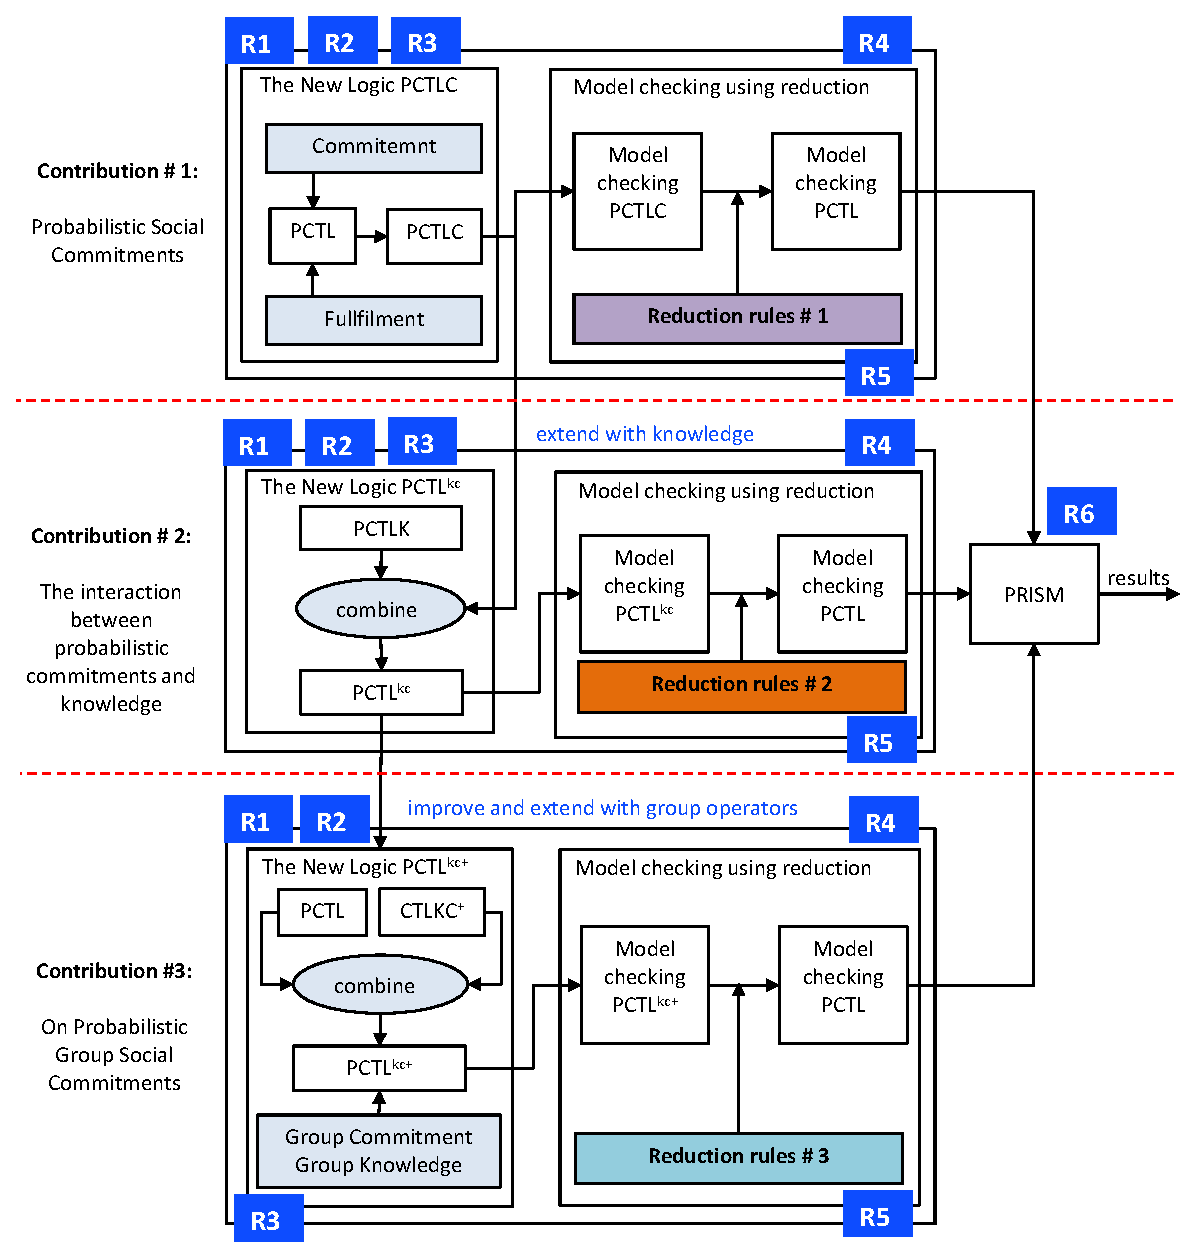
\includegraphics[width=16cm, height=20cm]{chap1/img/thesis-new.eps}
                \end{center}
                \caption{The Proposed Framework }
                \label{fig:proposed-framework}
    \end{figure}



To be able to handle social commitments when the scope of interacting agents is extended from the common one-to-one scheme to one-to-many scheme, we develop a semantics for the group social commitment operator and integrate it to the framework. We also add a group knowledge operator in order for the new logic to be more expressive and effective. The improved and refined logic is called the new logic of knowledge and commitments (PCTL$^{\textrm{kc+}}$). Moreover, we generalise the model checking technique proposed for PCTL$^{kc}$ to verify the new logic (PCTL$^{\textrm{kc+}}$) with the group operators.

Finally, each proposed reduction technique is implemented independently on top of the PRISM tool and applied to a concrete case study. 
Figure \ref{fig:proposed-framework} depicts the structure of the proposed work, links contributions to each other, and maps them to thesis chapters. Moreover, this figure shows where we answer each of the research questions presented in Section \ref{sec:problem statement-chap1}.




\section{Contributions}\label{sec:thesis-contributions-chap1}
We have developed a set of methods to pursue our objectives and to fill the research gap identified above. The majority of the work presented in this thesis has been published in the proceedings of various international conferences and refereed international journals. In summary, the main
contributions are:

\begin{enumerate}
\item A new logic called the probabilistic logic of commitments (PCTLC) that can represent and reason about social commitments in the presence of uncertainty \cite{Sultan2013}.

\item A new logic called the probabilistic logic of knowledge and commitment (PCTL$^{kc}$) whose expressive power helps capture the interaction between knowledge and social commitments in probabilistic MASs \cite{Sultan2014b}

\item A Semantics for group social commitment \cite{Sultan2014c}.

\item An improved version of the logic of knowledge and commitments enriched with epistemic and social group operators (PCTL$^{\textrm{kc+}}$). The distinguished feature of the new logic  lies in its ability of not only expressing the interaction between individual (basic) social commitments and knowledge, but also expressing the interaction between group social commitments and knowledge in the presence of uncertainty \cite{Sultan2014c}.

\item Three reduction-based model checking techniques for PCTLC \cite{Sultan2014a}, PCTL$^{kc}$ \cite{Sultan2014b}, and PCTL$^{\textrm{kc+}}$ \cite{Sultan2014d} respectively.

\item Implementation of the three proposed model checking techniques on top of the PRISM model checker using concrete case studies.

\end{enumerate}



\section{Thesis Organization}\label{sec:thesis-outline-chap1}
The remainder of this thesis is organized as follows. Chapter \ref{cha:background} describes the background needed for our research. Chapter \ref{cha:PCTLC}, presents a formal approach for handling probabilistic social commitments in MASs. In Chapter \ref{cha:PCTLKC}, we introduce a probabilistic approach for capturing and verifying the interaction between knowledge and social commitments. Chapter \ref{cha:PCTLKC+} presents an improved version of the approach presented in Chapter \ref{cha:PCTLKC} and then extends it to accommodate group knowledge and group commitments. %Also, in this chapter, a novel semantics for the group social commitment is given for the first time in the literature.
Chapter \ref{Chap5:Conclusion} concludes the thesis and identifies hints for future directions.


